%%%%%%%%%%%%%%%%%%%%%%%%%%%%%%%%%%%%%%%%%
% a0poster Portrait Poster
% LaTeX Template
% Version 1.0 (22/06/13)
%
% The a0poster class was created by:
% Gerlinde Kettl and Matthias Weiser (tex@kettl.de)
% 
% This template has been downloaded from:
% http://www.LaTeXTemplates.com
%
% License:
% CC BY-NC-SA 3.0 (http://creativecommons.org/licenses/by-nc-sa/3.0/)
%
%%%%%%%%%%%%%%%%%%%%%%%%%%%%%%%%%%%%%%%%%

%----------------------------------------------------------------------------------------
%	PACKAGES AND OTHER DOCUMENT CONFIGURATIONS
%----------------------------------------------------------------------------------------

\documentclass[a0,portrait]{a0poster}

\usepackage{multicol} % This is so we can have multiple columns of text side-by-side
\columnsep=100pt % This is the amount of white space between the columns in the poster
\columnseprule=3pt % This is the thickness of the black line between the columns in the poster

\usepackage[svgnames]{xcolor} % Specify colors by their 'svgnames', for a full list of all colors available see here: http://www.latextemplates.com/svgnames-colors

%\usepackage{times} % Use the times font
\usepackage{palatino} % Uncomment to use the Palatino font
\usepackage{plain} %bibliography style
\usepackage{graphicx} % Required for including images
\graphicspath{{figures/}} % Location of the graphics files
\usepackage{booktabs} % Top and bottom rules for table
\usepackage[font=small,labelfont=bf]{caption} % Required for specifying captions to tables and figures
\usepackage{amsfonts, amsmath, amsthm, amssymb} % For math fonts, symbols and environments
\usepackage{wrapfig} % Allows wrapping text around tables and figures
\usepackage{url}

\begin{document}

%----------------------------------------------------------------------------------------
%	POSTER HEADER 
%----------------------------------------------------------------------------------------

% The header is divided into two boxes:
% The first is 75% wide and houses the title, subtitle, names, university/organization and contact information
% The second is 25% wide and houses a logo for your university/organization or a photo of you
% The widths of these boxes can be easily edited to accommodate your content as you see fit

\begin{minipage}[b]{0.75\linewidth}
\veryHuge \color{NavyBlue} \textbf{Private Eye} \color{Black}\\ % Title
\Huge\textit{An ANN Based Computer Vision API}\\[2cm] % Subtitle
\huge \textbf{Theodoros Nikopoulos-Exintaris}\\[0.5cm] % Author(s)
\huge Aberystwyth University Computer Science\\[0.4cm] % University/organization
\Large \texttt{thn2@aber.ac.uk}\\
\end{minipage}
%
\begin{minipage}[b]{0.25\linewidth}

\includegraphics[width=20cm]{logo.png}\\
\end{minipage}

\vspace{1cm} % A bit of extra whitespace between the header and poster content

%----------------------------------------------------------------------------------------

\begin{multicols}{2} % This is how many columns your poster will be broken into, a portrait poster is generally split into 2 columns


%----------------------------------------------------------------------------------------
%	INTRODUCTION
%----------------------------------------------------------------------------------------

\color{SaddleBrown} % SaddleBrown color for the introduction

\section*{Introduction}

This project is concerned with the use of artificial neural networks and specifically deep convolutional neural networks for image classification. Its general aim is to investigate the performance of CNNs compared to other computer vision and types of ANN for this task as well as produce a simple wrapper API for interacting with the finished neural network which will be used to produce demonstration applications.

The ultimate goal of the project is to demonstrate the use of CNNs for image classification and hopefully multi-label classification and to then employ this technology to develop applications that will use such a technology.

%----------------------------------------------------------------------------------------
%	OBJECTIVES
%----------------------------------------------------------------------------------------

\color{DarkSlateGray} % DarkSlateGray color for the rest of the content

\section*{Main Objectives}

\begin{enumerate}
\item Decide on an ANN backend to use.
\item Develop a suitable ANN structure to train on the CIFAR-10 and MINST datasets to classify images.
\item Compare performance of different ANN structures for this problem
\item Create a suitable wrapper/API to for applications to interact with the ANN.
\item Develop simple web interface to submit images for classification to demonstrate the ANN working.
\item Extend to different demo applications and image classification problems.
\end{enumerate}

%----------------------------------------------------------------------------------------
%	MATERIALS AND METHODS
%----------------------------------------------------------------------------------------

\section*{Materials and Methods}

\section{Platform}
After investigating several tools and libraries like TensorFlow, we have decided to settle with the Keras Library with the Theono backend running on an nVidia GPU using CUDA.

This is largely because TensorFlow is currently lacking in critical platform support and is considered as of now an alpha release.

Keras was chosen because it is widely used and provides a very simple programming interface which greatly simplifies the prototyping of neural networks and training as well as performance measurement.

Theano is supported in Keras as a backend and is another widely used backend. It was chosen because of its speed and ease of use.

\section{Datasets}
We are using the MNIST and CIFAR-10 datasets to train our neural network these consist of several thousand small, under 40px images with associated labels which will be used for classification.

\subsection{MNIST}
This dataset is a reduced subset of the NIST handwritten digit database and is made up of 60,000 hand written digits for training examples and 10,000 testing examples. The dimensions of each image is 28x28px.

These are used as a proof of concept for the neural network and a successful model using this dataset should be able to recognise a wide variety of normalised hand-written digits.

\subsection{CIFAR-10}
This dataset is a smaller set of the CIFAR-100 dataset. It consists of 60,000 32x32 images organised into 10 classes hence its name. Each class is 6,000 images big and in addition contains 1,000 testing images per class for a total of 10,000 test images.

The CIFAR-100 dataset on the other hand contains the same number of images except we now have 100 classes of 600 training images and 20 superclasses for those 100 classes. Each class also includes 100 test images.
\begin{center}\vspace{1cm}
	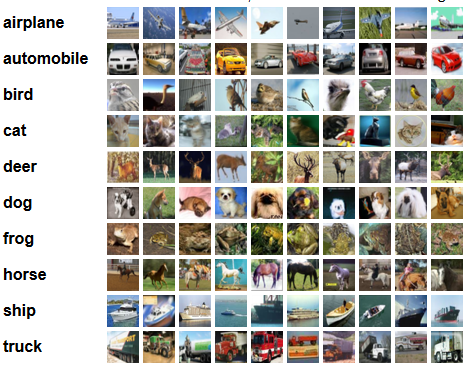
\includegraphics[width=0.8\linewidth]{cifar10}
	\captionof{figure}{\color{Green} Example of CIFAR-10 images taken from CIFAR website}
\end{center}\vspace{1cm}

\subsection{Network Structure}
The prime candidate for this task is a convolutional neural network. These types of networks have been found to work quite well with computer vision problems so our investigation has been largely oriented towards those.

Their structures tend to be quite simple and most if not all networks use a very similar application of an input layer followed by stripes of a convolution layer followed by a subsampling or pooling layer which is repeated until the desired network depth is reached. These are then mapped to a set of outputs which give use our ANN classification results.

\begin{center}\vspace{1cm}
	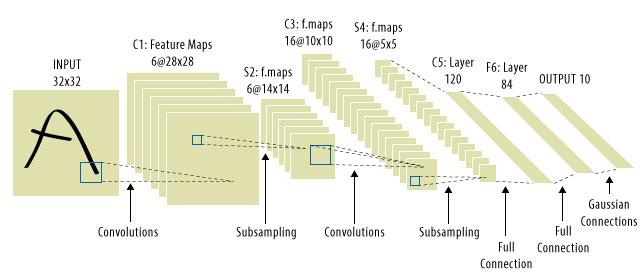
\includegraphics[width=0.8\linewidth]{common_cnn_design}
	\captionof{figure}{\color{Green} Example of a common CNN design. See acknowledgements}
\end{center}\vspace{1cm}

Convolution layers divide the visual field into smaller more manageable partitions while subsampling layers will merge inputs down. This is inspired by biological processes and on the assumption that interesting features tend to be very localised in the visual field so one only needs to consider parts of an image that are close together.

The main variables is the choice of weights, activation functions, convolution patterns and number of layers. These many variations will be tested throughout this project as well as other factors

\subsection{Testing Methods}
To evaluate the performance of our neural networks we will be using provided sets of test images which will then provide us with an accuracy for each experiment as well as appropriate tables. We will also try to benchmark our solutions with other people using the same data which is easy to do since CIFAR-10 is used to host competitions.

\section*{To The Future And Beyond}
By May I hope to achieve good performance on both CIFAR-10 and CIFAR-100 datasets which is meant to prove the viability of such a project. Once good ANN performance is achieved two ideas for demonstration apps include a site where images can be submitted to and classified. As well as perhaps advanced web crawlers that use ANN output to decide whether pictures are worth keeping or not based on a search query.

After May, I hope to move this project to my own dataset where I aim to build similar applications but on a larger scale and with images of a different nature. Ideally I would like to use this to classify large datasets of obtained images as well as equip existing datamining projects to be more 'inteligent' perhaps even implementing quality predictive functions. The site itself can be expanded to have user feedback evolving the project to an 'online' trained neural network.

 %----------------------------------------------------------------------------------------
%	REFERENCES
%----------------------------------------------------------------------------------------

\nocite{*} % Print all references regardless of whether they were cited in the poster or not
\bibliographystyle{IEEE}
\bibliography{mmp} % Use the example bibliography file sample.bib

%----------------------------------------------------------------------------------------
%	ACKNOWLEDGEMENTS
%----------------------------------------------------------------------------------------

\section*{Acknowledgements}
This Poster was produced in \LaTeX using the a0poster class:

 \(http://www.latextemplates.com/template/a0poster-portrait-poster\)
 
Figure 2 is taken from:

\(http://systemdesign.altera.com/can-you-see-using-convolutional-neural-networks/\)

%----------------------------------------------------------------------------------------

\end{multicols}
\end{document}